\documentclass{article}
\usepackage[margin=0.5in]{geometry}
\usepackage{siunitx}
\usepackage{amsthm}
\usepackage{amsmath}
\usepackage{tikz}
\usepackage{enumitem}

\title{4-1 Triangles Homework}
\date{}
\author{}

\begin{document}
\maketitle

\section*{Pythagorean Theorem}
For a right triangle with sides $a$, $b$, and $c$ where $a$ and $b$ meet to form a $\ang{90}$ angle and $c$ is the hypotenuse, $a^2 + b^2 = c^2$.

\begin{enumerate}
    \item If in $\triangle ABC$, $\angle A + \angle B = \ang{90}$, $AC = 4$, and $AB = 5$, what is $BC$?
        \vspace{3cm}
    \item A $25$-foot ladder is placed against a vertical wall.
        The foot of the ladder is $7$ feet from the base of the wall.
        If the top of the ladder slips $4$ feet, then how far will the foot slide?
        \vspace{3cm}
    \item An ant is crawling along the outside of the box.
        What is the distance he walks from $A$ to $B$ along the path shown?
        \begin{center}
            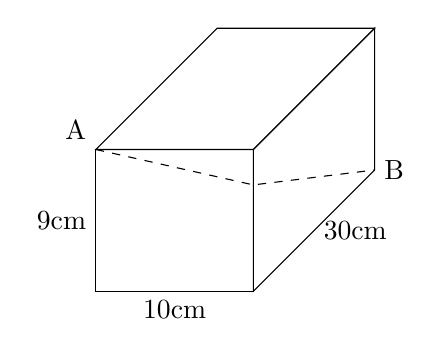
\begin{tikzpicture}
                \coordinate[label=above left:A] (A) at (0,1.8,4);
                \coordinate[label=right:B] (B) at (2,0,0);
                \draw (0,0,4) -- node[left] {9cm} (0,1.8,4) -- (A) -- (2,1.8,4) -- (2,0,4) -- node[below] {10cm} (0,0,4) -- cycle;
                \draw (B) -- node[right] {30cm} (2,0,4) -- (2,0,4) -- (2,1.8,4) -- (2,1.8,0) -- cycle;
                \draw (0,1.8,0) -- (2,1.8,0) -- (2, 1.8, 4) -- (A) -- cycle;
                \draw[dashed] (A) -- (2,1.35,4) -- (B);
            \end{tikzpicture}
        \end{center}
        \vspace{3cm}
\end{enumerate}

\newpage

\section*{Triangle Angle Sum}
The three angles in a triangle sum up to $\ang{180}$.

\begin{enumerate}[resume]
    \item In isosceles triangle $ABC$, $m\angle A = \ang{96}$.
        What is $m\angle B$?
        \vspace{3cm}
    \item The angle measures of a scalene triangle are $x$, $2x$ and $2x + 15$.
        What is the measure of the smallest angle?
        \vspace{3cm}
    \item What is the degree measure of angle $A$?
        \begin{center}
            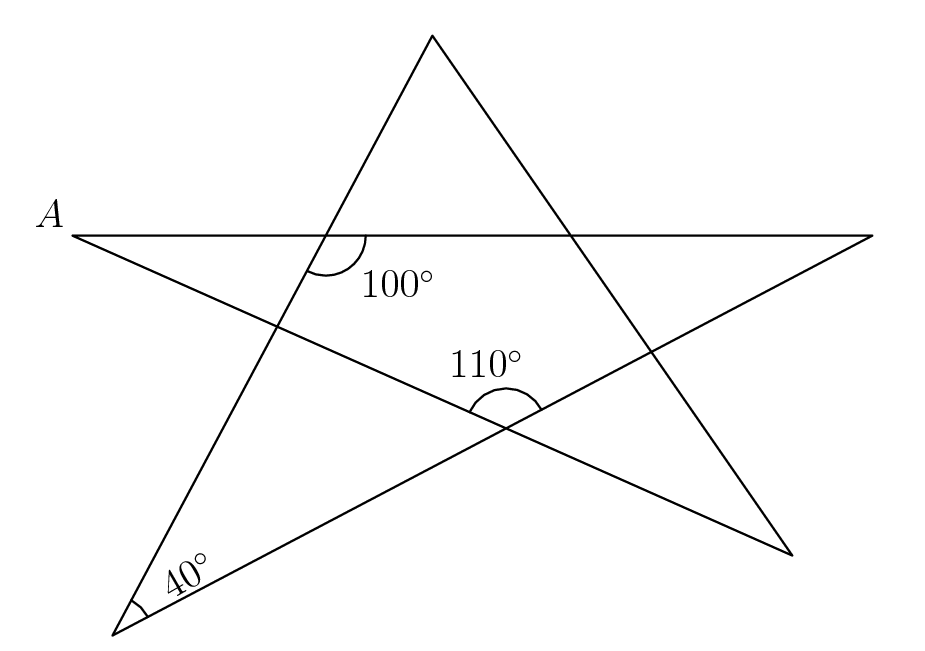
\includegraphics[scale=0.15]{star.png}
        \end{center}
        \vspace{3cm}
\end{enumerate}
\end{document}
